%%%%%%%%%%%%%%%%%%%%%%%%%%%%%%%%%%%%%%%%%%%%%%%%%%%%%%%%%%%%%%%%%%%%%
%% This is a (brief) model paper using the achemso class
%% The document class accepts keyval options, which should include
%% the target journal and optionally the manuscript type. 
%%%%%%%%%%%%%%%%%%%%%%%%%%%%%%%%%%%%%%%%%%%%%%%%%%%%%%%%%%%%%%%%%%%%%

\documentclass[journal=jacsat,manuscript=article]{achemso}
%\documentclass[journal=jacsat,manuscript=article]{achemso}

%%%%%%%%%%%%%%%%%%%%%%%%%%%%%%%%%%%%%%%%%%%%%%%%%%%%%%%%%%%%%%%%%%%%%
%% Place any additional packages needed here.  Only include packages
%% which are essential, to avoid problems later. Do NOT use any
%% packages which require e-TeX (for example etoolbox): the e-TeX
%% extensions are not currently available on the ACS conversion
%% servers.
%%%%%%%%%%%%%%%%%%%%%%%%%%%%%%%%%%%%%%%%%%%%%%%%%%%%%%%%%%%%%%%%%%%%%
\usepackage[version=3]{mhchem} % Formula subscripts using \ce{}
\usepackage{xargs}
\usepackage[colorinlistoftodos,prependcaption,textsize=tiny]{todonotes}

\usepackage[font=small,labelfont=bf]{caption}
%%%%%%%%%%%%%%%%%%%%%%%%%%%%%%%%%%%%%%%%%%%%%%%%%%%%%%%%%%%%%%%%%%%%%
%% If issues arise when submitting your manuscript, you may want to
%% un-comment the next line.  This provides information on the
%% version of every file you have used.
%%%%%%%%%%%%%%%%%%%%%%%%%%%%%%%%%%%%%%%%%%%%%%%%%%%%%%%%%%%%%%%%%%%%%
%%\listfiles

%%%%%%%%%%%%%%%%%%%%%%%%%%%%%%%%%%%%%%%%%%%%%%%%%%%%%%%%%%%%%%%%%%%%%
%% Place any additional macros here.  Please use \newcommand* where
%% possible, and avoid layout-changing macros (which are not used
%% when typesetting).
%%%%%%%%%%%%%%%%%%%%%%%%%%%%%%%%%%%%%%%%%%%%%%%%%%%%%%%%%%%%%%%%%%%%%
\newcommand*\mycommand[1]{\texttt{\emph{#1}}}

\newcommand{\figref}[2][]{\hyperref[#2]{Fig.~\ref{#2}#1}}
%%%%%%%%%%%%%%%%%%%%%%%%%%%%%%%%%%%%%%%%%%%%%%%%%%%%%%%%%%%%%%%%%%%%%
%% Place any additional packages needed here.  Only include packages
%% which are essential, to avoid problems later. Do NOT use any
%% packages which require e-TeX (for example etoolbox): the e-TeX
%% extensions are not currently available on the ACS conversion
%% servers.
%%%%%%%%%%%%%%%%%%%%%%%%%%%%%%%%%%%%%%%%%%%%%%%%%%%%%%%%%%%%%%%%%%%%%
\usepackage[version=3]{mhchem} % Formula subscripts using \ce{}

\setlength{\abovecaptionskip}{0pt}
\setlength{\belowcaptionskip}{-5pt}
\usepackage{gensymb}
\usepackage[version=3]{mhchem} % Formula subscripts using \ce{}
%\usepackage{hyperref}
\usepackage[normalem]{ulem}
\usepackage{textcomp}
\usepackage{color}
\usepackage{xcolor}
%\usepackage{pdfcomment}
\usepackage{amsmath}
\usepackage{amssymb}
\usepackage{pdfcomment}
\usepackage{paralist}

\usepackage{xargs}
\usepackage[colorinlistoftodos,prependcaption,textsize=tiny]{todonotes}

%\usepackage{float,rotating,subfigure}
\newcommandx{\commentPaul}[2][1=]{\todo[linecolor=red,backgroundcolor=red!25,bordercolor=red,#1]{#2}}
\newcommandx{\commentSajad}[2][1=]{\todo[linecolor=blue,backgroundcolor=blue!25,bordercolor=blue,#1]{#2}}
\newcommandx{\commentsAnthony}[2][1=]{\todo[linecolor=green,backgroundcolor=green!25,bordercolor=green,#1]{#2}}

\usepackage[font=small,labelfont=bf]{caption}
\usepackage{comment}

\defineavatar{Paul}{color=red}
\defineavatar{Sajad}{color=blue}

\bibliographystyle{achemso}
%%%%%%%%%%%%%%%%%%%%%%%%%%%%%%%%%%%%%%%%%%%%%%%%%%%%%%%%%%%%%%%%%%%%%
%% If issues arise when submitting your manuscript, you may want to
%% un-comment the next line.  This provides information on the
%% version of every file you have used.
%%%%%%%%%%%%%%%%%%%%%%%%%%%%%%%%%%%%%%%%%%%%%%%%%%%%%%%%%%%%%%%%%%%%%
%%\listfiles

%%%%%%%%%%%%%%%%%%%%%%%%%%%%%%%%%%%%%%%%%%%%%%%%%%%%%%%%%%%%%%%%%%%%%
%% Place any additional macros here.  Please use \newcommand* where
%% possible, and avoid layout-changing macros (which are not used
%% when typesetting).
%%%%%%%%%%%%%%%%%%%%%%%%%%%%%%%%%%%%%%%%%%%%%%%%%%%%%%%%%%%%%%%%%%%%%
%\newcommand*\mycommand[1]{\texttt{\emph{#1}}}

%%%%%%%%%%%%%%%%%%%%%%%%%%%%%%%%%%%%%%%%%%%%%%%%%%%%%%%%%%%%%%%%%%%%%
%% Meta-data block
%% ---------------
%% Each author should be given as a separate \author command.
%%
%% Corresponding authors should have an e-mail given after the author
%% name as an \email command. Phone and fax numbers can be given
%% using \phone and \fax, respectively; this information is optional.
%%
%% The affiliation of authors is given after the authors; each
%% \affiliation command applies to all preceding authors not already
%% assigned an affiliation.
%%
%% The affiliation takes an option argument for the short name.  This
%% will typically be something like "University of Somewhere".
%%
%% The \altaffiliation macro should be used for new address, etc.
%% On the other hand, \alsoaffiliation is used on a per author basis
%% when authors are associated with multiple institutions.
%%%%%%%%%%%%%%%%%%%%%%%%%%%%%%%%%%%%%%%%%%%%%%%%%%%%%%%%%%%%%%%%%%%%%

\author{Anthony J. Galante}
\affiliation[University of Pittsburgh]
{Department of Industrial Engineering, University of Pittsburgh, Pittsburgh, PA 15261, USA}
%\altaffiliation{A shared footnote}
%\author{Fred T. Secondauthor}
%\altaffiliation{Current address: Some other place, Othert\"own,
%Germany}

\author{Kathleen A. Yates}
\affiliation[University of Pittsburgh Medicine ]
{Department of Ophthalmology, Charles T. Campbell Laboratory for Ophthalmic Microbiology, University of Pittsburgh School of Medicine, Pittsburgh, PA 15213, USA}

\author{Brady Pilsbury}
\affiliation[University of Pittsburgh]
{Department of Industrial Engineering, University of Pittsburgh, Pittsburgh, PA 15261, USA}

\author{Melbs LeMieux}
\affiliation{7901 East Riverside Drive, Bldg 1,Unit 150, Austin TX  78744}

\author{Daniel J. Bain}
\affiliation[University of Pittsburgh]
{Department of Geology and Environmental Science, University of Pittsburgh, Pittsburgh, PA 15261, USA}

\author{Eric G. Romanowski}
%\altaffiliation{A shared footnote}
\affiliation[University of Pittsburgh Medicine]
{Department of Ophthalmology, Charles T. Campbell Laboratory for Ophthalmic Microbiology, University of Pittsburgh School of Medicine, Pittsburgh, PA 15213, USA}
%\phone{+123 (0)123 4445556}
%\fax{+123 (0)123 4445557}


\author{Robert M. Q. Shanks}
\affiliation[University of Pittsburgh Medicine ]
{Department of Ophthalmology, Charles T. Campbell Laboratory for Ophthalmic Microbiology, University of Pittsburgh School of Medicine, Pittsburgh, PA 15213, USA}


%\author{Christopher Matranga}
%\affiliation[National Energy Technology Laboratory (NETL)]
%{National Energy Technology Laboratory 626 Wallace Rd, Pittsburgh, PA 15236}


%\author{Congjun Wang}
%\affiliation[National Energy Technology Laboratory (NETL)]
%{National Energy Technology Laboratory 626 Wallace Rd, Pittsburgh, PA 15236}
%\email{s.k.laborator@bigpharma.co}
%\affiliation[BigPharma]
%{Lead Discovery, BigPharma, Big Town, USA}
\author{Paul W. Leu}
\affiliation[University of Pittsburgh]
{Department of Industrial Engineering, University of Pittsburgh, Pittsburgh, PA 15261, USA}
%\alsoaffiliation[Second University]
%{Department of Chemistry, Second University, Nearby Town}
\email{pleu@pitt.edu}

%%%%%%%%%%%%%%%%%%%%%%%%%%%%%%%%%%%%%%%%%%%%%%%%%%%%%%%%%%%%%%%%%%%%%
%% The document title should be given as usual. Some journals require
%% a running title from the author: this should be supplied as an
%% optional argument to \title.
%%%%%%%%%%%%%%%%%%%%%%%%%%%%%%%%%%%%%%%%%%%%%%%%%%%%%%%%%%%%%%%%%%%%%
\title
  {Bleach-durable reactive silver ink coatings for anti-viral, 
  %virucidal, 
  repellent, and reusable textiles}
% \title
%   {Comparison of virus killing durability after bleach washing of superhydrophobic, silver ink and silver nanoparticle coatings on PET for improving reusable PPE}

%%%%%%%%%%%%%%%%%%%%%%%%%%%%%%%%%%%%%%%%%%%%%%%%%%%%%%%%%%%%%%%%%%%%%
%% Some journals require a list of abbreviations or keywords to be
%% supplied. These should be set up here, and will be printed after
%% the title and author information, if needed.
%%%%%%%%%%%%%%%%%%%%%%%%%%%%%%%%%%%%%%%%%%%%%%%%%%%%%%%%%%%%%%%%%%%%%
\abbreviations{SEM,FTIR, PPE, GQDs, GO,  PET, NETL, ODA, PDMS}
\keywords{silver,killing, deactivation,anti-virofouling, virus, self-cleaning, superhydrophobic, reusable, personal protective equipment (PPE), fabric \LaTeX}

%%%%%%%%%%%%%%%%%%%%%%%%%%%%%%%%%%%%%%%%%%%%%%%%%%%%%%%%%%%%%%%%%%%%%
%% The manuscript does not need to include \maketitle, which is
%% executed automatically.
%%%%%%%%%%%%%%%%%%%%%%%%%%%%%%%%%%%%%%%%%%%%%%%%%%%%%%%%%%%%%%%%%%%%%
 \setlength {\marginparwidth }{2cm}
\begin{document}

%%%%%%%%%%%%%%%%%%%%%%%%%%%%%%%%%%%%%%%%%%%%%%%%%%%%%%%%%%%%%%%%%%%%%
%% The "tocentry" environment can be used to create an entry for the
%% graphical table of contents. It is given here as some journals
%% require that it is printed as part of the abstract page. It will
%% be automatically moved as appropriate.
%%%%%%%%%%%%%%%%%%%%%%%%%%%%%%%%%%%%%%%%%%%%%%%%%%%%%%%%%%%%%%%%%%%%%
\begin{tocentry}

Some journals require a graphical entry for the Table of Contents.
This should be laid out ``print ready'' so that the sizing of the
text is correct.

Inside the \texttt{tocentry} environment, the font used is Helvetica
8\,pt, as required by \emph{Journal of the American Chemical
Society}.

The surrounding frame is 9\,cm by 3.5\,cm, which is the maximum
permitted for  \emph{Journal of the American Chemical Society}
graphical table of content entries. The box will not resize if the
content is too big: instead it will overflow the edge of the box.

This box and the associated title will always be printed on a
separate page at the end of the document.

\end{tocentry}

%%%%%%%%%%%%%%%%%%%%%%%%%%%%%%%%%%%%%%%%%%%%%%%%%%%%%%%%%%%%%%%%%%%%%
%% The abstract environment will automatically gobble the contents
%% if an abstract is not used by the target journal.
%%%%%%%%%%%%%%%%%%%%%%%%%%%%%%%%%%%%%%%%%%%%%%%%%%%%%%%%%%%%%%%%%%%%%
\begin{abstract}
%During the most recent virus pandemic, the shortage of personal protective equipment (PPE) became a global health crisis. 
There is a major need to improve reusable personal protective equipment (PPE) with %virus inhibiting 
anti-viral
and liquid repelling functionality. %reusability  and durability for economical and environmental concerns. 
Silver is a popular coating material to incorporate virus inactivation functionality to PPE. This work consists of utilizing reactive silver inks and low surface energy polymers to achieve 
anti-viral and 
%enveloped virus inhibiting 
and liquid repellency functionalities even after ultrasonic bleach washing. The virus inhibition and repellency functionalities of reactive silver inks and silver nanoparticles on fabric are measured before and after bleach washing. The potential of reusability for reactive silver inks is compared with traditional silver nanoparticle coatings on fabric.
 
\end{abstract}

%%%%%%%%%%%%%%%%%%%%%%%%%%%%%%%%%%%%%%%%%%%%%%%%%%%%%%%%%%%%%%%%%%%%%
%% Start the main part of the manuscript here.
%%%%%%%%%%%%%%%%%%%%%%%%%%%%%%%%%%%%%%%%%%%%%%%%%%%%%%%%%%%%%%%%%%%%%
\section{Introduction}
%The shortage of PPE is a global health concern. Public spaces can be sources of infectious diseases during virus outbreaks when poor or no infection control measures are applied.\cite{querido_self-disinfecting_2019} Similarly, healthcare associated infections, when infections are spread to patients and employees in medical environments, affects millions of people and costs US hospitals billions of dollars each year. In hospitals, immunocompromised patients, healthcare workers and visitors can be exposed to high doses of infectious hazards, such as humancoronavirus severe acute respiratory syndrome coronavirus 2 (SARS-CoV-2), requiring the implementation of mitigation measures. A fomite is any inanimate object that becomes contaminated and has the capability to transfer disease to a new host. PPE commonly become fomites in hospitals and public spaces that spread disease. 

%Virus infections can be spread by virus particles within respiratory liquid droplets; therefore, the wetting property of PPE is very important. Surface wetting is described by the three phase interaction between solid, liquid and vapor phases that meet at the three-phase contact line. When a liquid droplet lands on a surface and the contact line is motionless, a static contact angle is formed from the interfacial surface tension forces acting along the solid-vapor, solid-liquid and liquid-vapor interfaces, represented by \(\gamma^{}_{SV}\),\(\gamma^{}_{SL}\) and \(\gamma^{}_{LV}\), respectively. The intrinsic static contact angle of a completely smooth surface, $\theta^{}_{Y}$, has the relationship $\cos{\theta^{}_{Y}} = \frac{\gamma^{}_{SV} - \gamma^{}_{SL}}{\gamma^{}_{LV}}$.\cite{young_thomas_iii._1805}.  The Cassie and Baxter equation describes the apparent contact angle when the surface roughness induces air pockets that make parts of the surface energetically unfavorable to be wet by liquid.\cite{cassie_wettability_1944}
%The equation derivation considers a composite interface between the surface and the entrapped air, where the entrapped air is assumed to be a fully liquid repellent surface layer.
%Therefore, the apparent contact angle of a composite surface with entrapped air $\theta^{}_{CB}$ may be defined by $\cos{\theta^{}_{CB}} = f_{1} \cos{\theta^{}_{Y}}+f_{1}-1 $, where $f_1$ is the fraction  of the surface area that is in contact with the liquid. %and $f_2$ is the fraction  of the surface area that is in contact with the air.
%$f_1 + f_2 = 1$ and $\theta_{Y_2} = 180$\degree~for air. 

%The amount of Laplace pressure required for liquid to infiltrate the air pockets and eliminate the Cassie-Baxter wetting state is called the breakthrough pressure. Breakthrough pressure can be experimentally calculated by observing the evaporation of a droplet on a surface. As the droplet evaporates, the Laplace pressure of the droplet on the surface increases. Breakthrough pressure is defined by
%\begin{equation}\label{eq:pressure}
%P(t) = 2 \gamma_{LV}/R(t)
%%   P = 2\gamma_{LV}/\sqrt{\gamma_{LV}/R}.
%\end{equation}
%where $\gamma_{LV}$ is liquid-vapor surface energy and R(t) is the radius of the droplet in contact with the surface\cite{Choi:17}. Breakthrough pressure is calculated by the size of the droplet when the evaporating droplet is observed to transition out of the Cassie-Baxter wetting state. 

%Surface wetting of droplets in motion can be characterized by the advancing contact angle, receding contact angle, and contact angle hysteresis. The advancing contact angle is the angle produced while a surface is being wetted; the receding angle is the contact angle where the surface has already been wetted and is in the act of dewetting. The advancing angle is always larger than or equal to the receding angle. The contact angle hysteresis is defined as 
%the advancing contact angle minus the receding contact angle. The contact angle hysteresis describes the tendency of a droplet to roll off when a surface is tilted.

%Surfaces can be engineered to achieve metastable Cassie-Baxter wetting states with outstanding liquid repellency properties. \cite{Chou:17,Hensel:springtail:16} Superhydrophobic surfaces 
%are defined as substrates that strongly repel water with
%static contact angles over 150$\degree$ and hysteresis less than 10$\degree$. Superhydrophobic repellency occurs when sufficient air is trapped between the water liquid and the surface that causes a spherical droplet to form as the thermodynamic energy on the surface is minimized.\cite{haghanifar_challenges_2020} Superhydrophobic surfaces have a self-cleaning property, where particulates on a surface can be removed by the liquid being fully repelled.

Personal protective equipment (PPE) such as  gowns,  masks, and scrubs are essential for protecting healthcare professionals from contact with bacteria and viruses that lead to infection.
% Viruses may also be transmitted via 
% respiratory droplets which can land on
%Respiratory droplets may also 
However, PPE may become contaminated during use and inadvertently contribute to the transmission of microbes \cite{Sakaguchi:10}. There is a need for textile coatings that provide PPE with better protection from infection 
%barrier properties by 
by not only repelling fluids such as 
respiratory droplets, but 
killing or deactivating microbes. In particular, there is great interest in textile coatings that provide these functionalities in reusable PPE even after laundering \cite{Kraay:18}.

Single-use or disposable PPE place a heavy burden on manufacturing supply chains that may lead to shortages during pandemics or times of great demand.\cite{cohen_contributing_2020}  
%\commentPaul{Find reference}
Single use or disposable PPE also lead to large amounts of waste and environmental impact \cite{Overcash:12}.
%Reusable PPE also 
%such as  gowns,  masks,  scrubs,  and  sheets  
%address these issues, 
Reusable PPE help alleviate burdens on manufacturing supply chains and decrease the amount of waste.  Furthermore, they are more economical on a cost per use basis.  \cite{Overcash:12} %\commentPaul{Find citation for this.}
However, one of the main challenges with reusable PPE is ensuring that they continue to provide protection from microbes after repeated use and decontamination.  Reusable PPE are decontaminated after each use by laundering with bleach.  
%are  subject to laundering with bleach for decontamination.  
% about 10\%  bleach  washing  for  20  min before being returned.\cite{cintas}
% There is a need for 
% improvements on the functionality and reusability of PPE for public health safety.\cite{Kraay:18} %Self-cleaning, medical coatings are a proactive strategy to prevent surface contamination from human body fluid, bacteria, and viruses.
% Reusable  PPE in the healthcare sector such as  gowns,  masks,  scrubs,  and  sheets  are  subject to  about 10\%  bleach  washing  for  20  min before being returned.\cite{cintas}
%, according  to  Cintas,  a  major  healthcare laundering  company. 
Therefore, virus inactivating surface coatings for reusable PPE in medical settings must be able to withstand multiple laundering cycles in bleach solution. 


% However, previous work on anti-microbial or anti-viral PPE applications neglect to analyze the durability of the functionality after washing with bleach. 
% \commentPaul{Some mention of bleach and its effects.}

Silver is a well-known anti-microbial agent.\cite{lansdown:06,Rai:09}
%for healthcare applications
 Previously, silver nanoparticles have been shown to inhibit the growth of yeast, \textit{Escherichia coli}, and \textit{Staphylococcus aureus}. \cite{Kim:07mar} %Silicon nanowires decorated with silver nanoparticles have been shown to have antimicrobial effect over 48 hours. \cite{lvm:10} 
%\commentPaul{Some examples with bacteria.}
More recently, silver nanoparticles have been demonstrated to have anti-viral properties against enveloped viruses such as severe acute respiratory syndrome coronavirus 2 (SARS-CoV-2) and human immunodeficiency viruses (HIV).\cite{jeremiah_potent_2020,lara_2010} 
Silver nanoparticles may interact with viral nucleic acids to disrupt serial viral infection and replication.\cite{jeremiah_potent_2020}
Silver nanoparticles have been incorporated into a range of 
fabrics or masks due to their anti-microbial and anti-viral properties.\cite{bu_fabrication_2019,perera_morphological_2013, lvm:10, zhong_plasmonic_2020,tremiliosi_ag_2020}
However, nanoparticles on fabrics may have issues with being removed in the wash, resulting in the loss of any associated functionality \cite{Lorenz:12,Impellitteri:09}.
%and other coatings 
%are easily , rendering the surface ineffective , and 
Washed out nanoparticles 
% that is washed out into the environment may 
%The use of silver may %be toxic, which may 
%cause harmful health side effects \cite{Sicherer:13,Stoker:10,Cunha:01} or
may also pose a threat to aquatic organisms \cite{Krysanov:10,Ma:13_nanoparticle,Fabrega:11,Pillai:14}
and bioaccumulate in the food chain \cite{Uddin:20}.
Also, the efficacy of silver nanoparticles may be hindered after washing with oxidizing agents such as bleach or detergent.\cite{lansdown:06}  

% Silver nanoparticles have strong efficacy against infectious hazards due to their large surface area for silver ions to diffuse.  
% Detergent wash durable antimicrobial properties have been shown using silver nanoparticles and an acrylic binder on cotton fabrics.  \cite{rojas-lema_2017} 



%Recently, silver has been proposed to have anti-viral properties against enveloped virus, such as SARS-CoV-2 and HIV.\cite{jeremiah_potent_2020,lara_2010} Silver nanoparticles interact with viral nucleic acids in a way that disrupts serial viral infection and replication.\cite{jeremiah_potent_2020} 
%Silver nanoparticles on fabrics have shown to prevent transmission and spread of SARS-CoV-2.\cite{tremiliosi_ag_2020} 

%Silver ink is a promising alternative for fabric treatments; however, the functionality durability of silver treated fabrics after bleach washing has not been investigated. 
% The use of silver for functional PPE applications must be durable so that 
% functionality is retained after repeated bleach washing.  
This work studies the virucidal activity of
PET textiles coated with a silver amine complex ink \cite{Walker:12}
on herpes simplex viruses (HSV-1).  
PET fabric material is commonly used for medical and healthcare applications such as gowns, scrubs and caps. \cite{Rigby:97} 
HSV-1 is an enveloped virus about 160 nm in diameter that can cause cold sores and blinding herpetic eye infections.\cite{wald:07} 
The attachment and entry of HSV-1 into cells requires the interaction between the viral envelope glycoproteins and cell surface heparan sulfate (HS).\cite{baram-pinto_2009} Silver mimics HS and competes for binding sites of the virus to the cell, inhibiting the virus from cell attachment and entry.\cite{baram-pinto_2009,Galdiero:11}

The virus inactivating activity of reactive silver ink or 20 nm silver nanoparticles against HSV-1 in saline is investigated.
Reactive silver ink in saline reduces HSV-1 activity by $1.6 \pm 0.9 \log_{10}$ ($90.3 \pm 5.5 \%$) while nanoparticles in saline did not show significant activity reduction.  
The virus quantities of PET fabrics coated with silver ink or silver nanoparticles is compared. Once the silver ink is cured, the additional ingredients evaporate leaving a pure silver film.  
PET fabrics coated with 20 nm silver nanoparticles %lose majority of its 
show a $1.1 \pm 0.6$ log$_{10}$ ($92.4 \pm 2.5 \%$, $p < 0.05$) log reduction in virus quantities compared to control fabric, 
while PET fabrics coated with reactive silver inks reduce virus quantities by $2.3 \pm 0.8$ log$_{10}$ ($99.5 \pm 3.0 \%$, $p < 0.001$). 
%The reduction of virus quantities on the fabric is likely from the liquid repellent properties, since both treatments render the fabric highly hydrophobic. The liquid containing the virus does not penetrate the treated fabric and a reduction of virus quantities is observed compared to controls. 
However, we observe the performance of bare silver fabric treatments can be significantly hindered after extended periods of bleach washing. 


%\commentPaul{Any ideas on the mechanism why reactive silver ink would be able to inactivate but silver nanoparticles not.}
%\commentPaul{Give percentage.}
%\commentPaul{Give $p$ number from t-test?}

%$2.3 \pm 0.8$ log, $2.7 \pm 0.8$ log, $2.7 \pm 0.8$ log and $2.8 \pm 0.7$ log PFU per mL, respectively.

We show that the reactive silver ink provides for enhanced washing durability compared to nanoparticles.  
Reactive silver reduces \textit{in-situ}
on the textile and uniformly covers 
%reduction and uniform silver coverage around 
the microfibers of the fabric.  
This provides for better binding with the fabric compared to nanoparticles, which adhere to the fabric with weak van der Waals forces.  
%for enhanced stability. 
% In this work, we compare the anti-viral properties of a reactive silver ink in phosphate buffered saline (PBS) and on polyester (PET) fabric with silver nanoparticles. 
An additional polydimethylsiloxane (PDMS) thin film can protect the silver layer and increase the liquid repellent properties or the fabric to improve %decontamination 
the durability of the functionality after decontamination by bleach washing. PET fabric samples coated with reactive silver ink and PDMS reduce virus quantities by $1.7 \pm 0.2$ log$_{10}$ ($98.2 \pm 0.8 \%$, $p < 0.01$) after 300 minutes of ultrasonic bleach washing. We demonstrate the combination of reactive silver inks with PDMS as a PET fabric treatment that adds durable superhydrophobic and virus reducing properties for reusable PPE applications. 


% Virus outbreaks cause significant social and economical burdens.\cite{Morens:13} The worldwide public health crisis of COVID-19 calls for reusable materials that repel and inactivate enveloped viruses for preventing transmission.\cite{rakowska_2021} Enveloped viruses have an outer viral envelope made of phospholipids, proteins and viral glycoproteins, and a capsid protein layer that encases the genome, consisting of deoxyribonucleic acid (DNA) or ribonucleic acid (RNA).\cite{chazal_2003} Examples of DNA species are herpesvirus (herpes), poxvirus (smallpox), and hepadnavirus (hepatits B), and RNA species are flavivirus (West Nile), orthomyxoviruses, (Influenza) and oronaviruses (SARS-CoV).\cite{rey_2018} 









%\cite{zhong_plasmonic_2020,zhong_reusable_2020,huang_self-reporting_2020} Carbon 2d nanomaterials such as graphene and graphene oxide are an emerging class of materials with antimicrobial effects theorized to be from mechanical damage and oxidative stress.\cite{liu_antibacterial_2011}
%Recent work using carbon 2d nanomaterials include superhydrophobic, reusable and recyclable graphene masks or self-reporting bacteria killing graphene masks, but did not perform experiments with virus. \cite{zhong_reusable_2020,huang_self-reporting_2020}
%Furthermore, reusable medical PPE must be durable after bleach washing, according to current washing protocols. 
%A superhydrophobic reduced GO and PDMS (polydimethylsiloxane) fabric coating showed excellent laundry durability up to 250 cycles, but did not use bleach nor perform functionality tests on viruses. \cite{yan_engineering_2016}
%Silver ions can diffuse through the PDMS thin film to inactivate viruses. 

% The treatment consists of a drop casting of silver ink, curing, followed by PDMS dip coating and subsequent curing. The PET fabric treatment is compared with 20 nm silver nanoparticles that are drop cast and heat sintered. An equal amount of 0.2 mg of silver is added to each fabric sample. 

 
\section{Results and discussion}

%0.2 mg of silver is added to PET fabric samples. 

\begin{figure}[H]
       \centering
    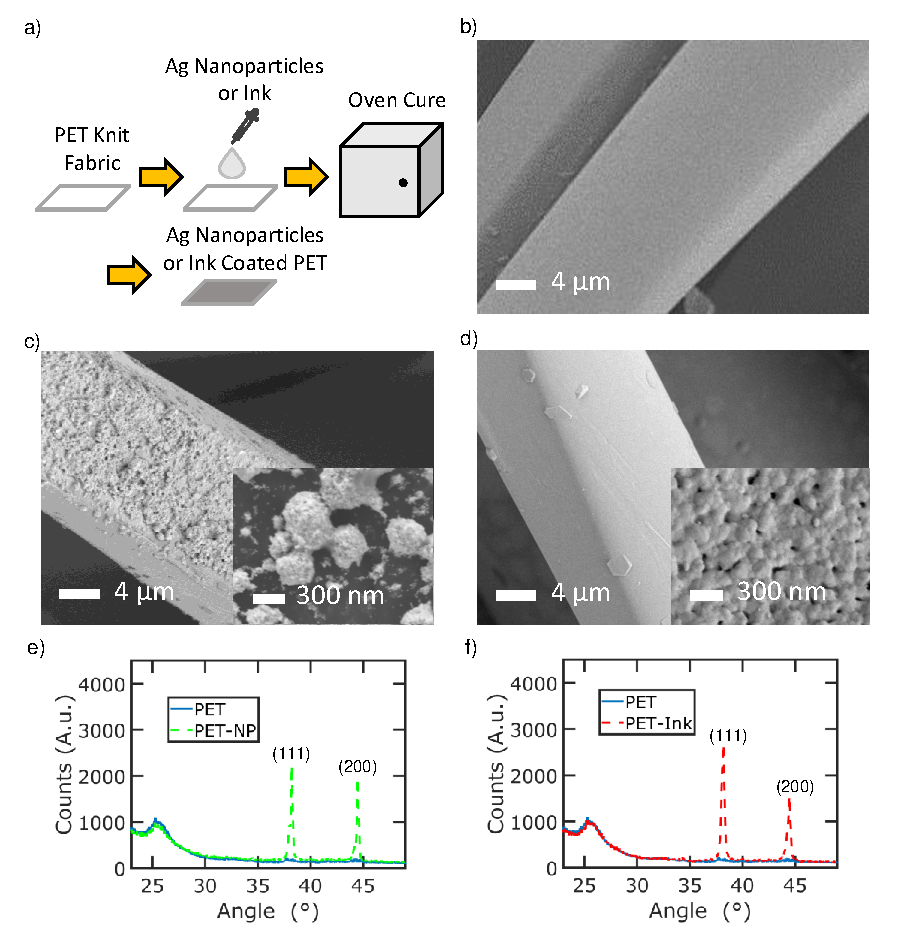
\includegraphics[width= \linewidth]{Figures/fig1_char.pdf}
   % \vspace{.1in}
   \caption[Scanning Electron Microscopy]{a) Schematic of silver treatment on PET fabric (b-d) SEM images of b) untreated PET c) PET-NP and d) PET-Ink. e-f) XRD spectra of e) PET-NP and f) PET-Ink samples.}
   %\commentPaul[inline]{Perhaps (c) and (d) should be (c)(i) and (ii).}
%    \commentPaul[inline]{Change text in (a) to ``Coat Ag Nanoparticles or Ink".}
    % \commentPaul[inline]{Add ``Ag Ink or Nanoparticle-Coated PET" to schematic.  Add another arrow (maybe two rows) with final sample.}
   %\commentPaul[inline]{Change text in (a) to ``Ag Nanoparticles or Ink".}
   %\commentPaul[inline]{Change (f) order to Control, NP, ink.  Make line in (i) and (ii) same blue color.  Change order of legend in (e) to PET and then with -NP and with -Ink.}
%   \commentPaul[inline]{Change line format so not overlapping so much.}
  
\label{fig:SEM}
\end{figure}

\figref{fig:SEM} shows the results of coating the PET fabric with silver nanoparticles or ink.  
The PET fabrics are coated by drop casting and then thermally cured
(\figref[a]{fig:SEM}).  Square fabric samples of 
0.5 in.~by 0.5 in are coated with either silver nanoparticles or ink by drop casting, followed by curing in an oven for 1 hour at 120 \degree C. An equal amount of silver by weight (0.2 mg) was added to each fabric. 
%An equal amount of 0.2 mg of silver isadded to each fabric sample. 
%\figref[b]{fig:SEM} shows scanning electron microscopy (SEM) images of 
The untreated PET knit fabric consist of microfibers about 12-15 \micro m in diameter (\figref[b]{fig:SEM}). %\figref[b]{fig:SEM} shows the nanoscale roughness after etching with KOH and KMn405. 
%\figref[c]{fig:SEM} shows SEM images of the PET fibers after they have been coated with 20 nm silver nanoparticles (PET-NP). 
The 20 nm silver nanoparticles (PET-NP) aggregate and attach non-uniformly over the surface of the PET (\figref[c]{fig:SEM}).  
%\figref[d]{fig:SEM} shows the 
In contrast, PET fibers %after they have been 
coated with silver ink (PET-Ink) 
is observed to be more uniform around the PET fibers (\figref[d]{fig:SEM}). 
%are shown in \figref[d]{fig:SEM}. The silver ink coating 
%\commentPaul{Sentence structure is a little repetitive.  Fig~ shows...  Used a lot throughout the paper.  Try to mix it up more.}
X-ray diffraction (XRD) is performed on the coated samples (\figref[e-f]{fig:SEM}). %shows X-ray diffraction (XRD) peaks of the silver coated PET
Distinct peaks are observed at 2$\theta =$ 38.2\degree and 44.5\degree corresponding to the (111) and (200) crystal planes. 
The XRD analysis confirms the presence of poly-crystalline silver on PET for nanoparticle (\figref[e]{fig:SEM}) and ink (\figref[f]{fig:SEM}) coatings, respectively. 



%\figref[f]{fig:SEM} demonstrates the surface chemistry of fabric samples. The entire spectra of PET samples are shown in (f)(i). Untreated PET samples have distinct hydrocarbon peaks at wavenumber 600, 1250, 1350, and 1850 cm-1. Etched PET samples introduce carbonyl groups at wavenumber 1650 cm-1, highlighted in (f)(ii). \cite{achagri_surface_2020} Etched PET GO-ODA samples show the presence of GO-ODA at 3100-3400 cm-1. Etched PET GO-ODA PDMS samples introduce additional methyl groups at 2800-2900 cm-1 on the surface. These peaks are highlighted in (f)(iii). The addition of methyl groups to the surface lowers the overall surface energy to improve repellency. 

\begin{figure}[H]
       \centering
    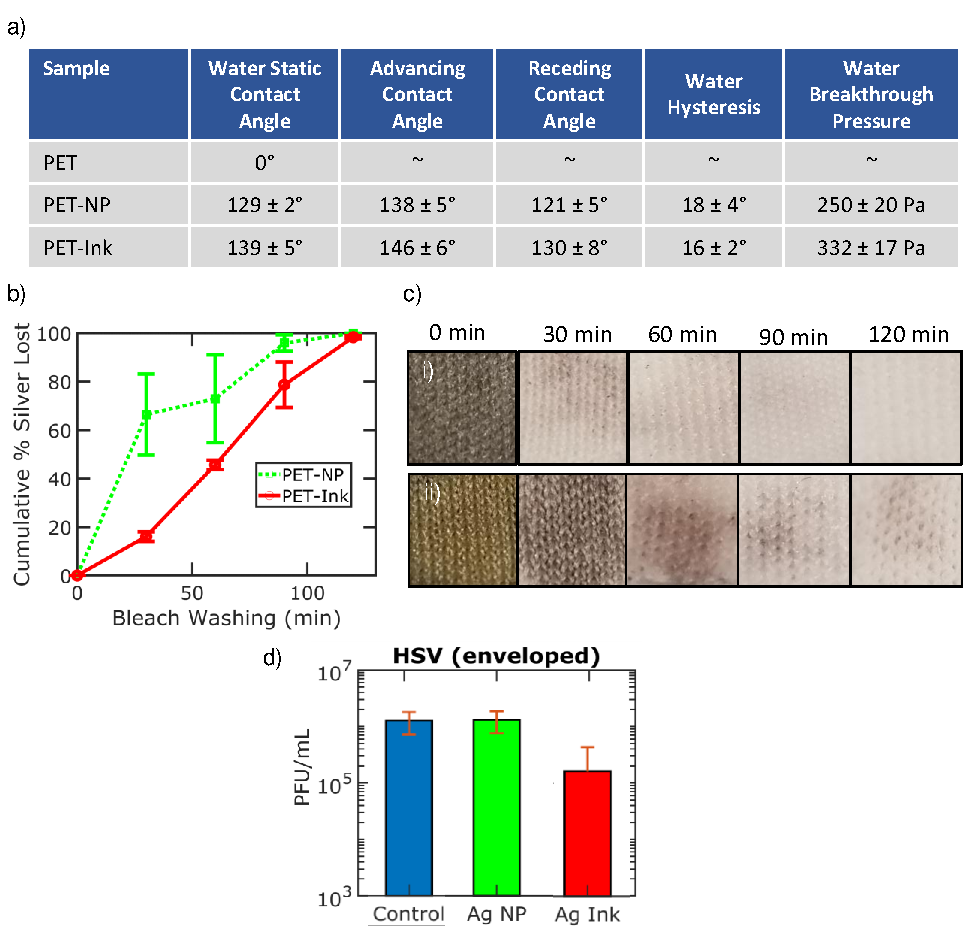
\includegraphics[width= \linewidth]{Figures/fig_wash1.pdf}
   % \vspace{.1in}
\caption[Durability]{
a) Wetting characterization for PET, PET-NP, and PET-Ink samples. b) Silver leaching analysis as a function of bleach washing time c) Optical images of (i) PET-NP and (ii) PET-Ink samples as a function of bleach washing time. d) Virus inhibition assay results of silver treatments in solution.} %FTIR spectra of etched PET GO-ODA + PDMS before and after 33 washes. e-f) Optical images of water (blue) and human saliva (yellow) droplets on i) EPGO and ii) EPGOP after (e) 250 abrasion cycles or (f) 33 bleach washing cycles.  %}
%\commentPaul[inline]{Perhaps change axes in (b) so max is 100 and min is 0.}
 %\commentsAnthony[inline]{i think it looks better with some space}
 %\commentPaul[inline]{The issue is that 0 and 100 are also the theoretical max and min.  I think you can change the plot so that the datapoint and error bar is on top of the axis if that is why you think it doesn't look good.}
 %\commentPaul[inline]{Maybe merge Table in (a) with Figure 1? (a) doesn't seem connected to rest of Figure.}
 %\commentPaul[inline]{Move 1(f) into this Figure as (d) to match order below.}

\label{fig:durable}
\end{figure}

\figref[a]{fig:durable} shows the wetting  properties of coated PET samples and virus inhibition properties of the silver coatings. Untreated PET is fully wetted by water. The water static contact angle and hysteresis of PET-NP is $129 \pm 2$\degree and $18 \pm 4$\degree, respectively. 
%\commentPaul{Perhaps want to reduce significant digits based on comment from other paper.}
The breakthrough pressure is estimated to be 
$250 \pm 20$ Pa based on the water droplet radius when the droplet transitions from a Cassie-Baxter state to a Wenzel state.  
%\commentPaul{Perhaps want to reduce significant digits of pressure too.}
%from an estimated droplet radius of 555 \micro m at breakthrough. 
The water static contact angle and hysteresis of PET-Ink is $139 \pm 5$\degree and $16 \pm 2$\degree, respectively. The breakthrough pressure is estimated to be $332 \pm 17$ Pa. 
%from an estimated droplet radius of 434 \micro m at breakthrough. 
Both coated PET samples show similar hydrophobic wetting properties due to the nanoscale roughness on microfibers. %PET-Ink samples show more robust wetting due to the uniformity of the coating. 

Bleach washing experiments were performed to assess the durability of silver.  
The cumulative percentage of silver that came off coated samples during bleach washing is shown in \figref[b]{fig:durable}. The silver concentration from the affluent of each 30 minute washing cycle was measured using inductively coupled plasma mass spectrometry (ICP-MS). PET-NP samples lose $62 \pm 9$\% of the coated silver after the first 30 minutes of washing. PET-Ink samples lose silver at a slower rate due to the more uniform coating and stronger attachment to the PET from the silver diamine complex. Both treatments lose at least 99\% of the silver by 120 minutes of washing. 
\figref[c]{fig:durable} shows representative images of the (i) PET-NP and (ii) PET-Ink samples as a function of bleach washing cycles.  
Bleach oxidizes silver, which degrades the intrinsic properties. It is evident that silver treated fabrics need additional surface treatment for reuse in bleach washing processes. 

Virus assays in saline are conducted by mixing silver ink or silver nanoparticles (0.1\%) in phosphate buffered saline (PBS) with HSV-1 in PBS for 1 hour, followed by centrifuging, removing the supernatant, and quantifying the amount of virus remaining. \figref[d]{fig:durable} shows the results of inactivation experiments of nanoparticle or reactive ink-coated PET  %-coated PET 
on enveloped HSV-1 in phosphate buffered saline (PBS) at a concentration of 1 mg per mL (0.1\%). 
While the 20 nm silver nanoparticles do not show HSV-1 inactivation with a $0.0 \pm 0.1$ log$_{10}$ difference, the silver ink shows HSV-1 inactivation in PBS by $1.6 \pm 0.9$ log$_{10}$ ($90.3 \pm 5.5 \%$) difference. 
%\commentPaul{Give percentage.}
Previous reports have suggested that virus inactivation is stronger with smaller diameter silver nanoparticles ($\leq$ 15 nm) and it is possible the nanoparticles are too large to cover the binding sites of HSV-1 to inhibit cell entry.\cite{jeremiah_potent_2020}
% It is possible the size of the nanoparticles are too large to cover the glycoprotein binding sites on the HSV envelope to inhibit virus activity. 
Also, the silver ink has additional components such as octylamine (5-10\%) and ammonium formate (1-5\%) which may contribute to the virus reduction. 
\commentPaul{Talk to Melbs about this.}
%Similarly, these reports use nanoparticles stabilized with the antibacterial polymer polyvinylpyrrolidone (PVP). The nanoparticles from this work are stabilized in sodium citrate solution, which may be the reason for the lack of virus inhibition activity observed in solution.
%\commentPaul{Citation or justification?}
%Also, the reactive ink consists of smaller silver ions for more virucidal activity compared to nanoparticles.  \commentPaul{Need to check this with Eric.  Not sure why reactive ink would have smaller ions compared to nanoparticles.}
 %\commentPaul{20 nm and 15 nm is not that different.}
 %\commentPaul{More explanation of possible differences?}



\begin{figure}[H]
       \centering
    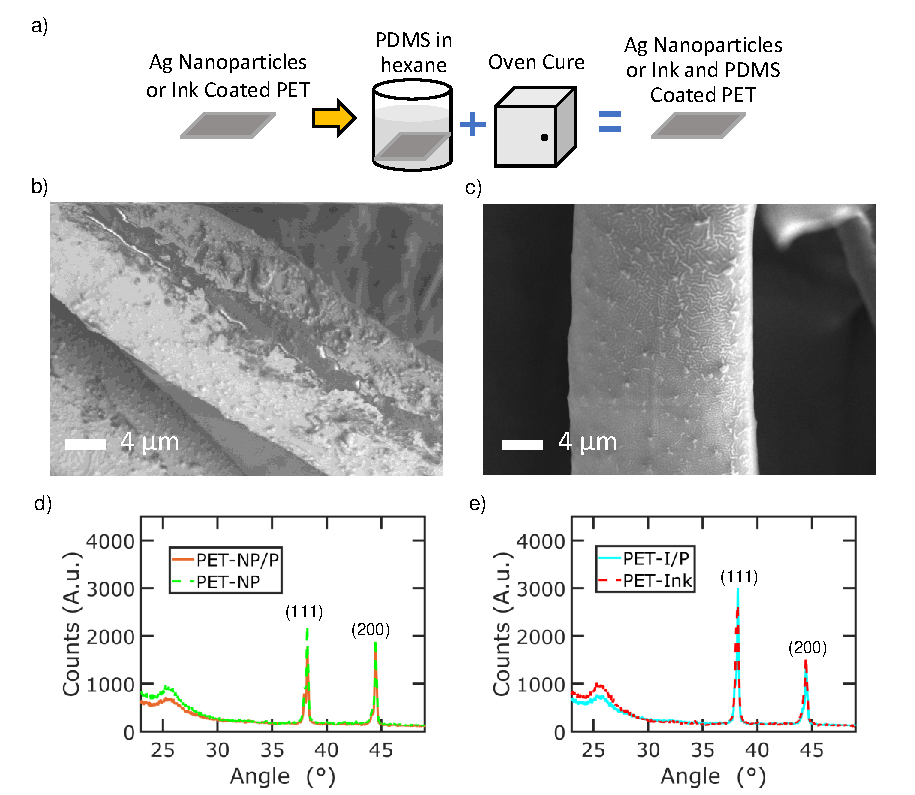
\includegraphics[width= \linewidth]{Figures/fig3_char.pdf}
   % \vspace{.1in}
\caption[SEM2]{a) Schematic of PDMS treatment for silver coated PET samples (b-c) SEM images of treated fiber of b) PET-NP/P and c) PET-I/P samples. d-e) XRD spectra of fabric samples before and after PDMS coating for d) PET-NP/P with PET-NP and e) PET-I/P with PET-Ink samples.}
   %\commentPaul[inline]{Change ``Ag Ink or Nanoparticles" to ``Ag Ink or Nanoparticle-Coated PET."}

   %\commentPaul[inline]{Show $+-$ as $\pm$.}
   %\commentPaul[inline]{Optical picture with water, saliva.}
   %\commentPaul[inline]{May want to move breakthrough pressure into supplement.}
%   \commentPaul[inline]{Orange seems a little too close to red.  Maybe pick another color.}
\label{fig:wet}
\end{figure}

A PDMS post treatment is added to the silver coated samples to improve the wash durability. PDMS is a low surface energy polymer that offers liquid repellent properties to fabrics.\cite{ye_2018} 
%\commentPaul{reference?}
Also, PDMS does not react heavily with bleach to add chemical resistance. Both PET-NP and PET-Ink samples are dipped in PDMS (1:10, Sylgard) and cured in an oven at 150 \degree C for two hours to make PET-NP/P and PET-I/P samples. 
%The PDMS coating improves the liquid repellency and silver retention of fabric samples.  
\figref{fig:wet} shows the characterization of PET-NP/P and PET-I/P samples. A schematic of the  PDMS treatment process is depicted in \figref[a]{fig:wet}.
%\commentPaul{Short description of process.  Follow template for Figure 1.  Use parentheses for all subfigures.}
%lists the water static contact angle, hysteresis and breakthrough pressure for respective samples. 
%\figref[b-c]{fig:wet} shows 
SEM imaging shows the physical morphology of microfibers for PET-NP/P (\figref[b]{fig:wet}) and PET-I/P (\figref[c]{fig:wet}) samples. The PDMS layer can be observed on the microfibers for both treatments. 
XRD spectroscopy identifies the crystalline phases present on PET-NP/P (\figref[d]{fig:wet}) and PET-I/P (\figref[e]{fig:wet}) microfibers before and after PDMS coating. The distinct silver peaks of (111) and (200) are still present for both samples after the PDMS coating, confirming the presence of silver on the samples. The PDMS coating adds broader peaks at 2$\theta =$ 22-27\degree due to the amorphous polymer structure. 
%\commentPaul{More discussion of difference without PDMS.}

\begin{figure}[H]
       \centering
    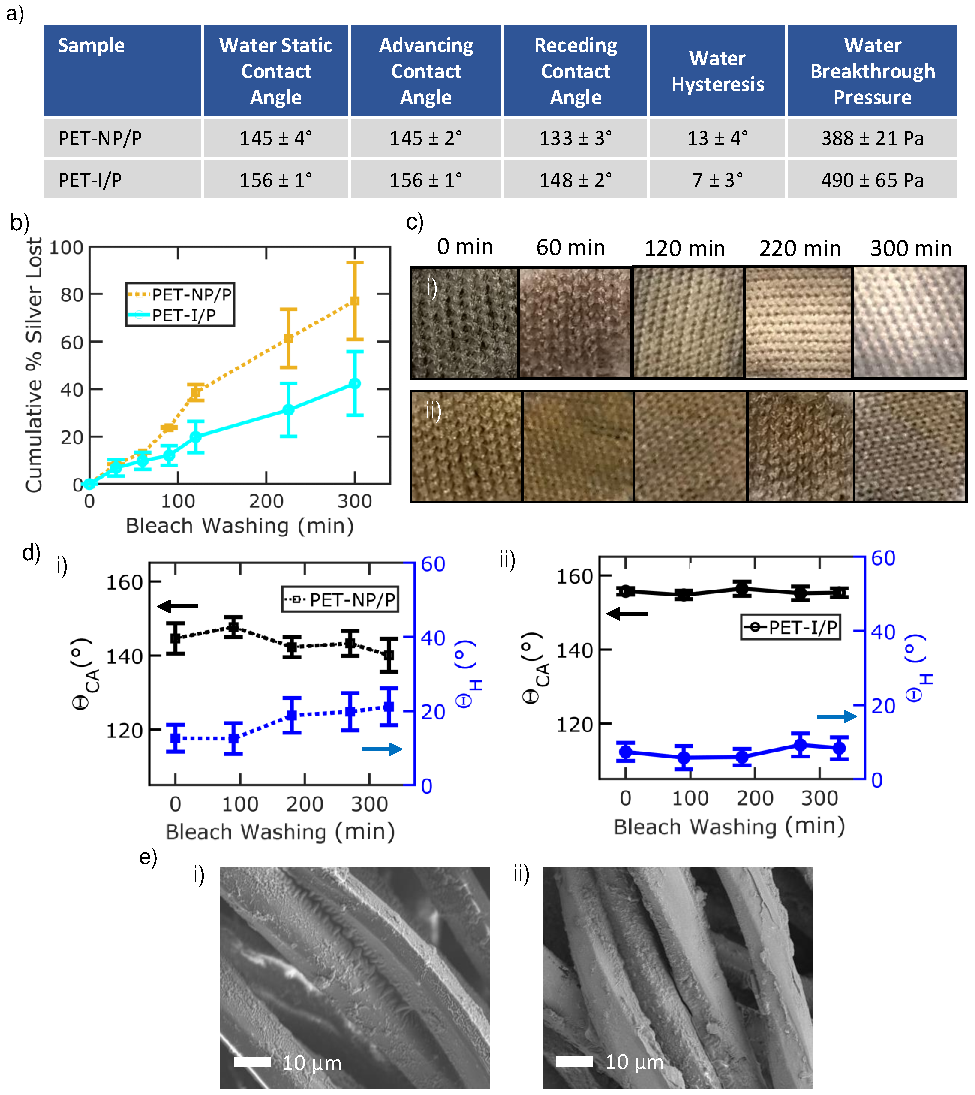
\includegraphics[width= \linewidth]{Figures/fig_wash2.pdf}
   % \vspace{.1in}
\caption[Durability]{a) Wetting characterization for PET-NP/P and PET-I/P samples b) Silver leaching analysis as a function of bleach washing time c) Optical images of (i) PET-NP/P and (ii) PET-I/P samples as a function of bleach washing time d) Water contact angle (black) and hysteresis (blue) as a function of ultrasonic bleach washing time for (i) PET-NP/P and (ii) PET-I/P}%FTIR spectra of etched PET GO-ODA + PDMS before and after 33 washes. e-f) Optical images of water (blue) and human saliva (yellow) droplets on i) EPGO and ii) EPGOP after (e) 250 abrasion cycles or (f) 33 bleach washing cycles.  }
%\commentPaul[inline]{Change arrows to black and blue.  Make arrow just pointing left and right, not diagonal.}
%\commentPaul[inline]{Same comment as before.  Probably want to move (a) to Figure 3.  }
\label{fig:durable2}
\end{figure}

\figref[a]{fig:durable2} shows the wetting properties of PET-NP/P and PET-I/P samples. The water static contact angle and hysteresis of PET-NP/P is $145 \pm 4$\degree and $13 \pm 4$\degree, respectively. The breakthrough pressure is $388 \pm 21$ Pa from an estimated droplet radius of 370 \micro m at breakthrough. The water static contact angle and hysteresis of PET-I/P is $156 \pm 1$\degree and $7 \pm 3$\degree, respectively. The breakthrough pressure is $490 \pm 65$ Pa from an estimated droplet radius of 294 \micro m at breakthrough. The PDMS layer significantly improves the liquid repellency properties of the fabrics for both treatments. PET-I/P demonstrates more water repellency than PET-NP/P due to the uniform, nanoscale roughness of the ink along all microfibers. PET-NP/P %\commentPaul{PET-NP/P?} 
samples are not uniformly covered by silver; therefore, there exists more fabric surface area without nanoroughness which leads to more liquid penetration. 
%\commentPaul{More discussion of difference without PDMS.}

The cumulative percentage of silver that came off PDMS coated samples during bleach washing is shown in \figref[b]{fig:durable2}. The additional PDMS layer of PET-NP/P and PET-I/P samples significantly improves the retention of silver compared to PET-NP and PET-Ink samples. The PDMS layer protects the silver layer from bleach oxidation and extends the washing durability of the samples. PET-NP/P samples lose more silver compared to PET-I/P samples. PET-I/P samples lose silver at a slower rate due to the stronger liquid repellency properties and higher breakthrough pressure. PET-I/P maintains about $42 \pm 17$\% more silver than PET-NP/P after 300 ultrasonic bleach washing minutes. 
\figref[c]{fig:durable2} shows representative images from (i) PET-NP/P and (ii) PET-I/P of the silver loss as a function of bleach washing cycles.  
PET-I/P retain color much better than PET-NP/P samples, which become stained from the bleach oxidizing and removing the silver.  
%\commentPaul{Also compare without the PDMS.}

\figref[d]{fig:durable2} illustrates the water static contact angle and hysteresis of (i) PET-NP/P and (ii) PET-I/P samples as a function of bleach washing time. The average change in static water contact angle and hysteresis for %uncured GO-ODA on PET fabric is $13.2 \pm 2.9$\degree and $17.6 \pm 2.4$\degree after only 6 bleach washing cycles. The average change in static water contact angle and hysteresis of EPGO 
PET-NP/P is $7 \pm 2$\degree and $9 \pm 1$\degree after 300 minutes of bleach washing. The average change in static water contact angle and hysteresis for 
PET-I/P is $1 \pm 1$\degree and $2 \pm 1$\degree after 300 minutes of bleach washing. The PDMS layer helps retain silver on PET samples during bleach washing; however, the PET-I/P coated samples show better performance and durability due to the stable liquid repelling properties. 

In this work, we measure the quantity of herpes simplex virus (HSV-1, enveloped) on fabrics, using standard plaque forming unit (PFU) assays, for samples that are unwashed, bleach washed for 100 minutes and bleach washed for 300 minutes samples.
%\commentPaul{It's a little odd that this is here because Fig.~1a showws inactivation experiments.  Probably should describe this by Fig.~1f.  Or move back here.}
Virus assays on fabric are conducted by submerging fabrics in virus/PBS while rocking for 1 hour, then samples are removed and placed in fresh PBS. Lastly, samples are sonicated at low power to remove viruses that adhered on the samples. The PBS liquid afterwards is used to quantify the amount of virus present on the samples. Mann-Whitney are utilized to offer a degree of statistical certainty that the fabric treatment reduces the amount of virus particles on the fabric compared to controls. Asterisks corresponds to the level of certainty that the treated samples are the same as the controls where one asterisk corresponds to $p \leq 0.05$, two for $p < 0.01$ and three for $p < 0.001$.

\begin{figure}[H]
       \centering
    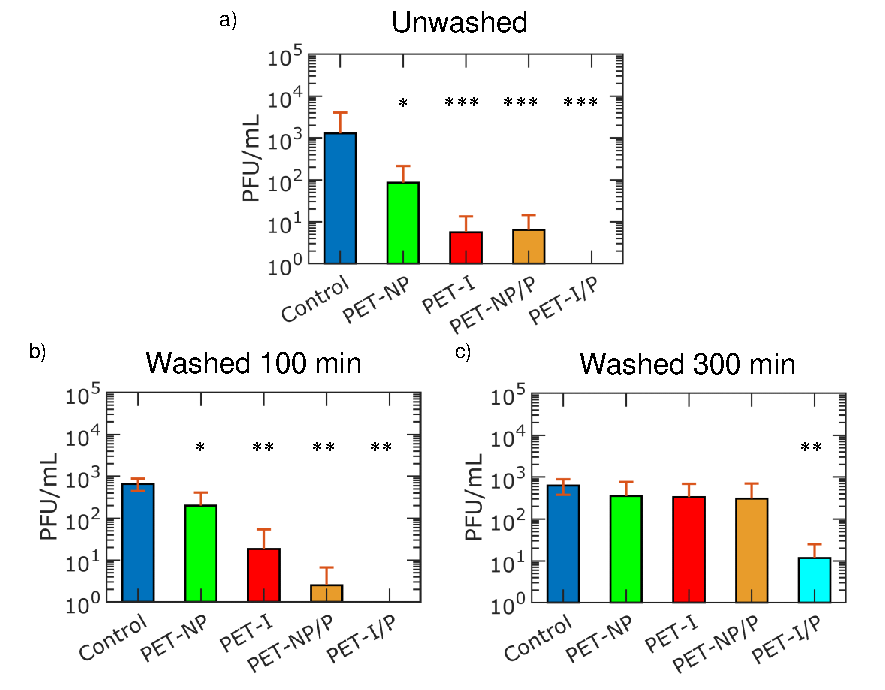
\includegraphics[width= \linewidth]{Figures/fig_virus.pdf}
    %\vspace{.5in}
\caption[Virus]{a) HSV-1 viral quantities for unwashed fabric samples b) HSV-1 viral quantities for fabric samples after 100 minutes of bleach ultrasonic washing c) HSV-1 viral quantities for fabric samples after 300 minutes of bleach ultrasonic washing. %Asterisks indicate the statistical certainty that the control is the same as the treatment from Mann-Whitney statistical tests, one asterisk for $p \leq 0.05$, two for $p < 0.01$ and three for $p < 0.001$.  
}

\label{fig:virus}
\end{figure}

%\vspace{.1in}
%\commentPaul{Representative plaques?}

The amount of virus on fabric samples before and after ultrasonic bleach washing is shown in \figref{fig:virus}. \figref[a]{fig:virus} shows the amount of active virus on unwashed fabric samples. PET-NP, PET-Ink, PET-NP/P and PET-I/P samples show a reduction of HSV-1 by $1.1 \pm 0.6$ log$_{10}$ ($92.4 \pm 2.5 \%$, $p < 0.05$), $2.3 \pm 0.8$ log$_{10}$ ($99.5 \pm 3.0 \%$, $p < 0.001$), $2.3 \pm 0.8$  log$_{10}$ ($99.5 \pm 3.1 \%$, $p < 0.001$) and $2.8 \pm 0.2$ log$_{10}$ ($99.8 \pm 0.9 \%$, $p < 0.001$) PFU per mL, respectively. 
%\commentPaul{Give percentages in parentheses.}
PDMS swells in the presence of liquid which potentially allows silver to slowly diffuse.\cite{bian_2021,ahmad_2021}
The reduction of activated virus is from a combination of liquid repellency and virus inactivation.  
% For nanoparticle coated fabrics, the reduction of virus is from the liquid repellent property. For ink coated fabrics, the reduction of virus is from a combination of liquid repellent property and the virus inhibition property.


The amount of virus on fabric samples after 100 minutes of bleach washing is shown in \figref[b]{fig:virus}. PET-NP, PET-I, PET-NP/P and PET-I/P samples show a reduction of HSV-1 by $0.6 \pm 0.4$ log$_{10}$ ($74.8 \pm 2.0 \%$, $p < 0.05$), $1.6 \pm 0.4$ log$_{10}$ ($97.2 \pm 1.9 \%$, $p < 0.01$), $2.4 \pm 0.3$ log$_{10}$ ($99.6 \pm 1.0 \%$, $p < 0.01$) and $2.8 \pm 0.1$ log$_{10}$ ($99.8 \pm 0.4 \%$, $p < 0.01$) PFU per mL,  respectively. Samples without the PDMS layer lose some functionality as significant amounts of the silver is removed from washing. Samples with the PDMS layer maintain liquid repellency and silver after 100 minutes of bleach washing due to the chemical resistance of PDMS which retains the silver layer. 

%PET-Ink samples show a reduction of virus by $626.7 \pm 227.2$ PFU per mL ($2.8 \pm 0.2$ log). PET-NP/P samples show a reduction of virus by $657.5 \pm 195.8$ PFU per mL ($2.8 \pm 0.1$ log) from the liquid repellency properties. PET-I/P samples show a reduction of virus by $660.0 \pm 198.9$ ($2.8 \pm 0.1$ log) PFU per mL. 

Lastly, the amount of virus on fabric samples after 300 minutes of bleach washing is shown in \figref[c]{fig:virus}. PET-NP, PET-I samples and PET-NP/P samples no longer show statistically significant reductions in HSV-1 after this extended bleach washing time from a lack of silver and liquid repellency properties. PET-I/P samples after 300 minutes of bleach washing still show a reduction of virus by $1.7 \pm 0.2$ log$_{10}$ ($98.2 \pm 0.8 \%$, $p < 0.01$) PFU per mL by the liquid repellency and virus inactivation properties. %It is likely after 300 minutes of bleach washing, more of the silver ink layer is exposed and the virus reduction is comparable to unwashed PET-Ink samples. 
Overall, the PET-I/P treated fabrics reduce the amount of active virus, even after 300 minutes of bleach washing. The ink coating covers the fibers more uniformly and the PDMS coating adds silver retention and liquid repellent properties for reusable, anti-viral performance.
% \commentPaul{Any papers showing that silver can diffuse through PDMS?}
% \commentsAnthony{a papers show that organic 
% molecules can diffuse through pdms membranes, a 
% paper suggesting water vapor can permeate through 
% nanopores in pdms (papers in allrefs zotero under 
% tags pdms diffusion}


\subsection{Conclusion}
%Virus infections cause a significant economical and social burden. 
There is a need for reusable, functional PPE to improve the public health safety against viral infections. This work demonstrates how %coal based carbon nanomaterials 
silver ink and low surface energy polymers can be used to repel liquid and inactivate viruses on polyester fabric with long lasting functionality. The fabric treatment fully repels water before and after bleach washing. Most importantly, the fabric treatment shows reductions in enveloped virus quantities by about 2 logs compared to controls before and after bleach washing. %The treatment is fluorine-free and utilizes cheap coal stocks for the potential of large scale production. 
This work demonstrates a durable, superhydrophobic, virus inactivating functionality on common fabric for reusable PPE applications.



%\subsection{Outline}

%The document layout should follow the style of the journal concerned.
%Where appropriate, sections and subsections should be added in the
%normal way. If the class options are set correctly, warnings will be
%given if these should not be present.

%\subsection{References}

%The class makes various changes to the way that references are
%handled.  The class loads \textsf{natbib}, and also the
%appropriate bibliography style.  References can be made using
%the normal method; the citation should be placed before any
%punctuation, as the class will move it if using a superscript
%citation style
%\cite{Mena2000,Abernethy2003,Friedman-Hill2003,EuropeanCommission2008}.
%The use of \textsf{natbib} allows the use of the various citation
%commands of that package: \citeauthor{Abernethy2003} have shown
%something, in \citeyear{Cotton1999}, or as given by
%Ref.~\citenum{Mena2000}.  Long lists of authors will be
%automatically truncated in most article formats, but not in
%supplementary information or reviews \cite{Pople2003}. If you
%encounter problems with the citation macros, please check that
%your copy of \textsf{natbib} is up to date. The demonstration
%database file \texttt{achemso-demo.bib} shows how to complete
%entries correctly. Notice that ``\latin{et al.}'' is auto-formatted
%using the \texttt{\textbackslash latin} command.

%Multiple citations to be combined into a list can be given as
%a single citation.  This uses the \textsf{mciteplus} package
%\cite{Johnson1972,*Arduengo1992,*Eisenstein2005,*Arduengo1994}.
%Citations other than the first of the list should be indicated
%with a star. If the \textsf{mciteplus} package is not installed,
%the standard bibliography tools will still work but starred
%references will be ignored. Individual references can be referred
%to using \texttt{\textbackslash mciteSubRef}:
%``ref.~\mciteSubRef{Eisenstein2005}''.

%The class also handles notes to be added to the bibliography.  These
%should be given in place in the document \bibnote{This is a note.
%The text will be moved the the references section.  The title of the
%section will change to ``Notes and References''.}.  As with
%citations, the text should be placed before punctuation.  A note is
%also generated if a citation has an optional note.  This assumes that
%the whole work has already been cited: odd numbering will result if
%this is not the case \cite[p.~1]{Cotton1999}.

\begin{comment}

\subsection{Floats}

New float types are automatically set up by the class file.  The
means graphics are included as follows (Scheme~\ref{sch:example}).  As
illustrated, the float is ``here'' if possible.
\begin{scheme}
  Your scheme graphic would go here: \texttt{.eps} format\\
  for \LaTeX\, or \texttt{.pdf} (or \texttt{.png}) for pdf\LaTeX\\
  \textsc{ChemDraw} files are best saved as \texttt{.eps} files:\\
  these can be scaled without loss of quality, and can be\\
  converted to \texttt{.pdf} files easily using \texttt{eps2pdf}.\\
  %\includegraphics{graphic}
  \caption{An example scheme}
  \label{sch:example}
\end{scheme}

\begin{figure}
  As well as the standard float types \texttt{table}\\
  and \texttt{figure}, the class also recognises\\
  \texttt{scheme}, \texttt{chart} and \texttt{graph}.
  \caption{An example figure}
  \label{fgr:example}
\end{figure}

Charts, figures and schemes do not necessarily have to be labelled or
captioned.  However, tables should always have a title. It is
possible to include a number and label for a graphic without any
title, using an empty argument to the \texttt{\textbackslash caption}
macro.

The use of the different floating environments is not required, but
it is intended to make document preparation easier for authors. In
general, you should place your graphics where they make logical
sense; the production process will move them if needed.

\subsection{Math(s)}

The \textsf{achemso} class does not load any particular additional
support for mathematics.  If packages such as \textsf{amsmath} are
required, they should be loaded in the preamble.  However,
the basic \LaTeX\ math(s) input should work correctly without
this.  Some inline material \( y = mx + c \) or $ 1 + 1 = 2 $
followed by some display. \[ A = \pi r^2 \]

It is possible to label equations in the usual way (Eq.~\ref{eqn:example}).
\begin{equation}
  \frac{\mathrm{d}}{\mathrm{d}x} \, r^2 = 2r \label{eqn:example}
\end{equation}
This can also be used to have equations containing graphical
content. To align the equation number with the middle of the graphic,
rather than the bottom, a minipage may be used.
\begin{equation}
  \begin{minipage}[c]{0.80\linewidth}
    \centering
    As illustrated here, the width of \\
    the minipage needs to allow some  \\
    space for the number to fit in to.
    %\includegraphics{graphic}
  \end{minipage}
  \label{eqn:graphic}
\end{equation}

\end{comment}

\section{Experimental}


\subsection{Sample Preparation}
Materials: PET knit wipes were purchased from Anticon. Acetone (99.5\%), methanol (99.9\%) and isopropyl alcohol (99.5\%) were bought from VWR.  PBS, FBS, PDMS (Sylgard) and were bought from Sigma-Aldrich. Reactive silver inks (720 series) was provided by Electroninks. Silver nanoparticles (20 nm, 1mg/mL Citrate) were purchased from NanoComposix. Household bleach was purchased from Giant Eagle. Deionized water was used from a Millipore Academic A10 system with total organic carbon below 40 ppb. Herpes simplex virus were obtained from the American Type Culture Collection (ATCC), Manassas, VA. Virus stocks in PBS were prepared with A549 human lung carcinoma cells and were cesium chloride centrifuge purified to remove any cellular and FBS proteins. The virus stocks were diluted in sterile PBS to the experimental titers used.

Sample Fabrication: 0.5 in.~by 0.5 in.~square samples were cut from PET fabric. All samples were rinsed with acetone, methanol and isopropyl alcohol and dried with nitrogen to eliminate possible contaminants. An equal amount of 0.2mg of silver was added to fabric samples, confirmed by microscale. Silver ink was added by drop casting onto untreated PET fabrics followed by oven curing for 1 hour at 120 \degree C to make PET-Ink samples. Silver nanoparticles was added by drop casting onto untreated PET fabrics followed by oven curing for 1 hour at 120 \degree C to make PET-NP samples. Additional PET-Ink and PET-NP samples were treated with a PDMS layer by soaking samples in PDMS (Sylgard) at 1:10 curing agent  ratio and curing for two hours at 150 \degree C to make PET-I/P and PET-NP/P samples, respectively. 

\subsection{Sample Characterization}
The physical morphologies of samples were characterized by scanning electron microscopy (SEM, Zeiss Sigma 500 VP) at 5kV. For SEM imaging, all samples were sputter coated with 10 nm gold/palladium (80:20) using a sputter coater (Denton). The presence of silver was confirmed used X-ray diffraction (XRD). %The chemical compositions of samples were characterized by Fourier transform infrared spectroscopy (FTIR, Bruker Vertex-70LS) between 600 and 3200 cm−1 wavelengths. 

Static, advancing and receding contact angle measurements were taken in ambient air at 22–25°C and 20–30\% relative humidity using an optical tensiometer (Attension, 811 Theta). 5 \micro L droplets at 25°C for all test liquids were used for all wetting measurements. The hysteresis was tabulated for each treatment after measuring the advancing and receding contact angles during syringe-controlled water dispersion and withdrawal, respectively.

Breakthrough pressure was measured by observing the contact angle and volume while a water droplet evaporates. When the droplet transitioned from Cassie-Baxter to Wenzel state the diameter of the droplet was tabulated to calculate the breakthrough pressure.



\subsection{Durability Testing}

%Mechanical abrasion tests were performed using Taber Linear or Rotary Abrader (Model 5750) under Ford Laboratory Test Method standards for resistance to abrasion of textile treatments (BN 108-02).  Samples were fixed on a stage and subject to abrasion cycles. 

Washing cycles were performed using a Powersonic P230 Ultrasonic Cleaner (Crest) under ASTM G131-96 standards for washing materials by ultrasonic techniques. 10\% bleach washing solution was prepared in a 10 mL test tube to create a highly efficient washing solution. Samples were submerged in bleach solution in Eppendorf tubes and ultrasonicated for 30 minutes at 80 W and 54°C to complete one wash cycle. Afterwards, samples were dried in ambient temperature before testing.

Silver leaching analysis was conducted using inductively coupled plasma-mass spectrophotometer (ICP-MS). Wash affluent was collected as samples were subject to bleach washing cycles. Then, samples were diluted for ICP-MS by mixing 9.8 mL of water (2\% nitrate solution), 10 \micro L of standard and 20 \micro L of wash affluent and taking the weights using a microscale. The weights were used to calculate dilution factors for ICP-MS results. 


\subsection{Virus Assays}
Virus inactivation assays were performed by mixing silver nanoparticles or silver ink with  herpes virus in PBS at final concentration of 1 mg per mL (0.1\%). Solutions were vortexed and incubated for 1 hour %while shaking for 60 minutes (Stoval Belly Dancer, level 7) 
at room temperature. After 1 hour of incubation, 500 \micro l of ice-cold tissue culture media containing 20\% FBS was added, then vortexed and centrifuged for 1 minute in the Eppendorf centrifuge to pellet any silver. The supernatants were removed and plated with 0.1 ml of serial 10-fold dilutions in duplicate onto A549 monolayers in 24 well multiplates. The virus was absorbed for 1-3 hours after which the wells were filled with 1 ml of tissue culture media containing 0.5\% methyl cellulose.  Plates were incubated for 5-6 days in 5\% CO2 and then fixed and stained with 0.5\% gentian violet solution containing formalin and the plaques were quantified.

Assays on Fabrics: Fabric samples were completely submerged in 0.4 mL of virus/PBS in Eppendorf tubes with moderate shaking for 60 minutes (Stoval Belly Dancer, level 5) at room temperature. %Adenovirus/PBS inoculum titers were averaged as 1.6x105 and 1.4x104 PFU mL−1 for types 4 and 7a viruses, respec-tively. 
After shaking, samples were gingerly rinsed once in sterile PBS and submerged in Eppendorf tubes with 0.4 mL of PBS. Then, virions attached on the surface were removed from the samples into PBS by sonication at power 3 for 10 seconds (Qsonica, Model Q55) within the tubes. The remaining PBS was used to quantify plaques. 

Virus titers (PFU per mL) for herpes simplex virus were determined using standard plaque assay with A549 human lung carcinoma cells prepared in 24-well tissue culture plates. After 6-7 days incubation at 37°C in 5\% CO2, the cells were fixed and stained with gentian violet prepared in formalin, the number of plaques per well were counted under a dissecting microscope, and viral plaque forming unit titers were calculated. 
%Betacoronavirus (CoV) OC43 titers were determined using tissue culture infectious dose 50 (TCID50) method with A549 human lung carcinoma cells prepared in 96-well tissue culture plates. After 14-16 days of incubation at 37°C in 5\% CO2, the cells were fixed and stained with gentian violet, wells were examined at 100x using the inverted microscope and a plus or negative sign is added depending on the cytopathic effect. Then, TCID50 cacluater was used to determine the titer of stock in TCID50 per ml. 
Finally, Mann-Whitney U-tests rejected the null hypothesis at p values $<$ 0.05 for all comparisons between control and treated samples.

%The usual experimental details should appear here.  This could
%include a table, which can be referenced as Table~\ref{tbl:example}.
%Notice that the caption is positioned at the top of the table.
%%\begin{table}
 % \caption{An example table}
  %\label{tbl:example}
 % \begin{tabular}{ll}
 %   \hline
  %  Header one  & Header two  \\
  %  \hline
  %  Entry one   & Entry two   \\
   % Entry three & Entry four  \\
  %  Entry five  & Entry five  \\
   % Entry seven & Entry eight \\
    %\hline
 % \end{tabular}
%%\end{table}


\begin{comment}


Adding notes to tables can be complicated.  Perhaps the easiest
method is to generate these using the basic
\texttt{\textbackslash textsuperscript} and
\texttt{\textbackslash emph} macros, as illustrated (Table~\ref{tbl:notes}).
\begin{table}
  \caption{A table with notes}
  \label{tbl:notes}
  \begin{tabular}{ll}
    \hline
    Header one                            & Header two \\
    \hline
    Entry one\textsuperscript{\emph{a}}   & Entry two  \\
    Entry three\textsuperscript{\emph{b}} & Entry four \\
    \hline
  \end{tabular}

  \textsuperscript{\emph{a}} Some text;
  \textsuperscript{\emph{b}} Some more text.
\end{table}


The example file also loads the optional \textsf{mhchem} package, so
that formulas are easy to input: \texttt{\textbackslash ce\{H2SO4\}}
gives \ce{H2SO4}.  See the use in the bibliography file (when using
titles in the references section).

The use of new commands should be limited to simple things which will
not interfere with the production process.  For example,
\texttt{\textbackslash mycommand} has been defined in this example,
to give italic, mono-spaced text: \mycommand{some text}.

\section{Extra information when writing JACS Communications}

When producing communications for \emph{J.~Am.\ Chem.\ Soc.}, the
class will automatically lay the text out in the style of the
journal. This gives a guide to the length of text that can be
accommodated in such a publication. There are some points to bear in
mind when preparing a JACS Communication in this way.  The layout
produced here is a \emph{model} for the published result, and the
outcome should be taken as a \emph{guide} to the final length. The
spacing and sizing of graphical content is an area where there is
some flexibility in the process.  You should not worry about the
space before and after graphics, which is set to give a guide to the
published size. This is very dependant on the final published layout.

You should be able to use the same source to produce a JACS
Communication and a normal article.  For example, this demonstration
file will work with both \texttt{type=article} and
\texttt{type=communication}. Sections and any abstract are
automatically ignored, although you will get warnings to this effect.

\end{comment}

%%%%%%%%%%%%%%%%%%%%%%%%%%%%%%%%%%%%%%%%%%%%%%%%%%%%%%%%%%%%%%%%%%%%%
%% The "Acknowledgement" section can be given in all manuscript
%% classes.  This should be given within the "acknowledgement"
%% environment, which will make the correct section or running title.
%%%%%%%%%%%%%%%%%%%%%%%%%%%%%%%%%%%%%%%%%%%%%%%%%%%%%%%%%%%%%%%%%%%%%
\begin{acknowledgement}

%Please use ``The authors thank \ldots'' rather than ``The
%authors would like to thank \ldots''.
The authors thank Dr.~Ke Ren for his statistical expertise. 
%The authors thank Dr. Richard A. Wolfe from Carbon Technology Co. (Bristol, VA) for providing the coal char. The nanographene oxide synthesis, functionalization and characterization were carried out by Dr. Viet Hung Pham, Dr. Jennifer Weidman, Dr. Congjun Wang, and Dr. Christopher Matranga at the National Energy Technology Laboratory. The authors thank Dr. Viet Hung Pham, Dr. Jennifer Weidman, Dr. Congjun Wang, and Dr. Christopher Matranga for their help and expertise.
%Mats Dahlgren for version one of \textsf{achemso},
%and Donald Arseneau for the code taken from \textsf{cite} to move
%citations after punctuation. Many users have provided feedback on the
%class, which is reflected in all of the different demonstrations
%shown in this document.

\end{acknowledgement}

%%%%%%%%%%%%%%%%%%%%%%%%%%%%%%%%%%%%%%%%%%%%%%%%%%%%%%%%%%%%%%%%%%%%%
%% The same is true for Supporting Information, which should use the
%% suppinfo environment.
%%%%%%%%%%%%%%%%%%%%%%%%%%%%%%%%%%%%%%%%%%%%%%%%%%%%%%%%%%%%%%%%%%%%%
\begin{suppinfo}

%This will usually read something like: ``Experimental procedures and
%characterization data for all new compounds. The class will
%automatically add a sentence pointing to the information on-line:
Virus inactivation experiment results, goniometer images of static water contact angles of fabric samples, XRD spectra and SEM images of PDMS treated fabric samples after bleach washing. 


\end{suppinfo}

%%%%%%%%%%%%%%%%%%%%%%%%%%%%%%%%%%%%%%%%%%%%%%%%%%%%%%%%%%%%%%%%%%%%%
%% The appropriate \bibliography command should be placed here.
%% Notice that the class file automatically sets \bibliographystyle
%% and also names the section correctly.
%%%%%%%%%%%%%%%%%%%%%%%%%%%%%%%%%%%%%%%%%%%%%%%%%%%%%%%%%%%%%%%%%%%%%
\bibliography{achemso-demo,AllRefs}

\end{document}